\documentclass[12pt,a4paper]{article}
\usepackage{amsmath,amscd,amsbsy,amssymb,latexsym,url,bm,amsthm}
\usepackage{epsfig,graphicx,subfigure}
\usepackage{enumitem,balance}
\usepackage{wrapfig}
\usepackage{mathrsfs,euscript}
\usepackage[usenames]{xcolor}
\usepackage{hyperref}
\usepackage[vlined,ruled,linesnumbered]{algorithm2e}
\hypersetup{colorlinks=true,linkcolor=black}

\newtheorem{theorem}{Theorem}
\newtheorem{lemma}[theorem]{Lemma}
\newtheorem{proposition}[theorem]{Proposition}
\newtheorem{corollary}[theorem]{Corollary}
\newtheorem{exercise}{Exercise}
\newtheorem*{solution}{Solution}
\newtheorem{definition}{Definition}
\theoremstyle{definition}
\pdfoptionpdfminorversion=6
\renewcommand{\thefootnote}{\fnsymbol{footnote}}

\newcommand{\postscript}[2]
 {\setlength{\epsfxsize}{#2\hsize}
  \centerline{\epsfbox{#1}}}

\renewcommand{\baselinestretch}{1.0}

\setlength{\oddsidemargin}{-0.365in}
\setlength{\evensidemargin}{-0.365in}
\setlength{\topmargin}{-0.3in}
\setlength{\headheight}{0in}
\setlength{\headsep}{0in}
\setlength{\textheight}{10.1in}
\setlength{\textwidth}{7in}
\makeatletter \renewenvironment{proof}[1][Proof] {\par\pushQED{\qed}\normalfont\topsep6\p@\@plus6\p@\relax\trivlist\item[\hskip\labelsep\bfseries#1\@addpunct{.}]\ignorespaces}{\popQED\endtrivlist\@endpefalse} \makeatother
\makeatletter
\renewenvironment{solution}[1][Solution] {\par\pushQED{\qed}\normalfont\topsep6\p@\@plus6\p@\relax\trivlist\item[\hskip\labelsep\bfseries#1\@addpunct{.}]\ignorespaces}{\popQED\endtrivlist\@endpefalse} \makeatother

\begin{document}
\noindent

%========================================================================
\noindent\framebox[\linewidth]{\shortstack[c]{
\Large{\textbf{Lab02-Divide and Conquer}}\vspace{1mm}\\
CS214-Algorithm and Complexity, Xiaofeng Gao, Spring 2019.}}
\begin{center}
\footnotesize{\color{red}$*$ If there is any problem, please contact TA Jiahao Fan.}

% Please write down your name, student id and email.
\footnotesize{\color{blue}$*$ Name:\_\_\_\_\_\_\_\_\_  \quad Student ID:\_\_\_\_\_\_\_\_\_ \quad Email: \_\_\_\_\_\_\_\_\_\_\_\_}
\end{center}

\begin{enumerate}
    \item
    Consider the following recurrence:
    \begin{equation*}
    T(n)=
    \begin{cases}
    \ 0 & \text{if } n=1 \\
    \ 2T(n/2)+O(n\log{n}) & \text{if } n=2^k \text{ and } k \geq 1 \\
    \end{cases}
    \end{equation*}
    \begin{enumerate}
        \item
        Solve $T(n)$ (in the form of $O$-notation) by recurrence tree. Detailed derivation is required.
%        \begin{solution}
%            Uncomment this block to write your solution.
%        \end{solution}

        \item
        Can we use the Master Theorem to solve this recurrence? Please explain your answer.
%        \begin{solution}
%            Uncomment this block to write your solution.
%        \end{solution}

    \end{enumerate}

    \item
    Given any array $num$, find the number of pairs $(i, j)$ satisfying $i < j$ and $num[i] > 2 \times num[j]$. For example, if $num=[1,3,2,3,1]$, the answer should be 2.
    \begin{enumerate}
        \item
         Design an algorithm to solve this problem using divide-and-conquer strategy and complete the implementation in the provided C/C++ source code. {\color{blue}(The source code \emph{Code-Pairs.cpp} is attached on the course webpage.)}

        \item
        Write a recurrence for the running time of your algorithm and solve it using the Master Theorem directly.
%        \begin{solution}
%            Uncomment this block to write your solution.
%        \end{solution}
    \end{enumerate}

    \item
    \textbf{Transposition Sorting Network}: A comparison network is a \textbf{transposition network}  if each comparator connects adjacent lines, as in the network in Fig.~\ref{Fig-Transposition}.

    \begin{figure}[htbp]
        \caption{A}
        \centering
        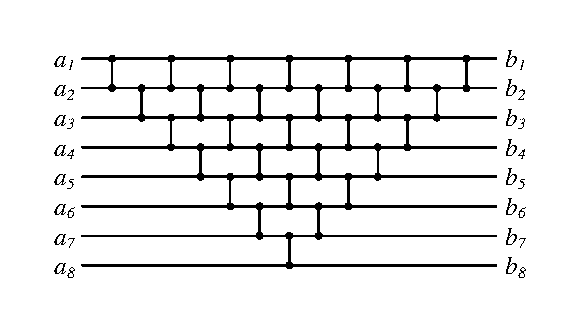
\includegraphics[width=0.5\textwidth]{Fig-Transposition.pdf}
        
        \label{Fig-Transposition}

    \end{figure}
    
    \begin{enumerate}
        \item
        Prove that a transposition network with $n$ inputs is a sorting network if and only if it sorts the sequence $\langle n, n-1, \cdots, 1 \rangle$. {\color{blue}(Hint: Use an induction argument analogous to the \emph{Domain Conversion Lemma}.)}
%        \begin{proof}
%           Uncomment this block to write your proof.
%        \end{proof}

        \item
        {\color{red}{(Bonus)}} Given any $n \in \mathbb{N}$, write a program using Tkinter in Python to draw a figure similar to Fig.~\ref{Fig-Transposition} with $n$ input wires.
        
    \end{enumerate}

\end{enumerate}

\vspace{20pt}

\textbf{Remark:} include your .cpp, .py, .pdf and .tex files in your uploaded .rar or .zip file.

%========================================================================
\end{document}
